% Template for TALYS school: In no way do you have to use this for your report. 
% It also helps you with what headings you can use- AGAIN you DO NOT have to use them- or change them to what you want. You should just try to cover what was lectured 
%Also just shows you some basic latex: includes how to add figures, table, citations. 
%Remember your report needs to be 5-10 pages of text. With as many figures as you want. 
% We require your report to have a 
%1. Introduction
%2. Some theory (nuclear physics and nuclear astrophysics)
%3. How elements are created
%4. NLD and GSF 
%5 Experiments to study
%6. Nuclear reaction model codes: TALYS
%7. TALYS exercises and discussion of the results
%8. Conclusion and outlook 
%9. Bibliography


\documentclass[english, notitlepage]{article}
\usepackage[utf8]{inputenc}
\usepackage{unicode-math}
\usepackage{graphicx}
\usepackage{babel}
\usepackage[version=4]{mhchem} 
\usepackage[a4paper, top=3cm, bottom=3cm, left=3cm, right=3cm]{geometry}
\usepackage{float}
\usepackage[format=plain,
            font=it]{caption} % Italicizes figure captions
\usepackage{csquotes}
\usepackage{geometry}
 \geometry{a4paper,
 total={170mm,257mm},
 left=25mm,
 top=25mm,} % Formats the paper size, orientation, and margins
\linespread{1.25} % about 1.5 spacing in Word
\usepackage{mhchem}
\setlength{\parindent}{0pt} % no paragraph indents
\setlength{\parskip}{1em}
\usepackage[backend=biber,citestyle=numeric-comp,sorting=none,sortcites,hyperref=true]{biblatex}
\usepackage[colorlinks=true]{hyperref} % For hyperlinks in the document
% Allows you to do citations - does Harvard style and compatible with Zotero
% Ensures the names of the authors after the first author are in the correct order in the bibliography% Corrects punctuation for authors with just a first initial. 
%When you are citing in text you use the \cite{keyword}.
\addbibresource{references.bib} %This is the name of your file that contains your references in bibtex form. 
\usepackage[format=plain,
            font=it]{subcaption} % Italicizes figure captions
\geometry{letterpaper, portrait, margin=1in}
\usepackage[format=plain,
            font=it]{caption} % Italicizes figure captions
\setlength{\headheight}{14.49998pt}

\title{INTPART summer school, 2025}

\author{Your name goes here}

\begin{document}
\maketitle
\begin{abstract}
A short overview of what your report is about.
\end{abstract}

% Here you can introduce what a 
\section{Introduction}

\section{Nuclear physics and nuclear astrophysics}

%If you want to bullet things you can use enumerate: This gives the number list. If you want unnumbered you can use: \begin{itemize} and then \end{itemize}
\begin{enumerate}
    \item How you add bullets
    \item Add a new bullet
\end{enumerate}



\subsection{Elements and their production in the Solar System}
\subsection{Nuclear Burning stages of stars}
\subsection{The production of heavy nuclei}

%How to insert a figure
\begin{figure}
    \centering
    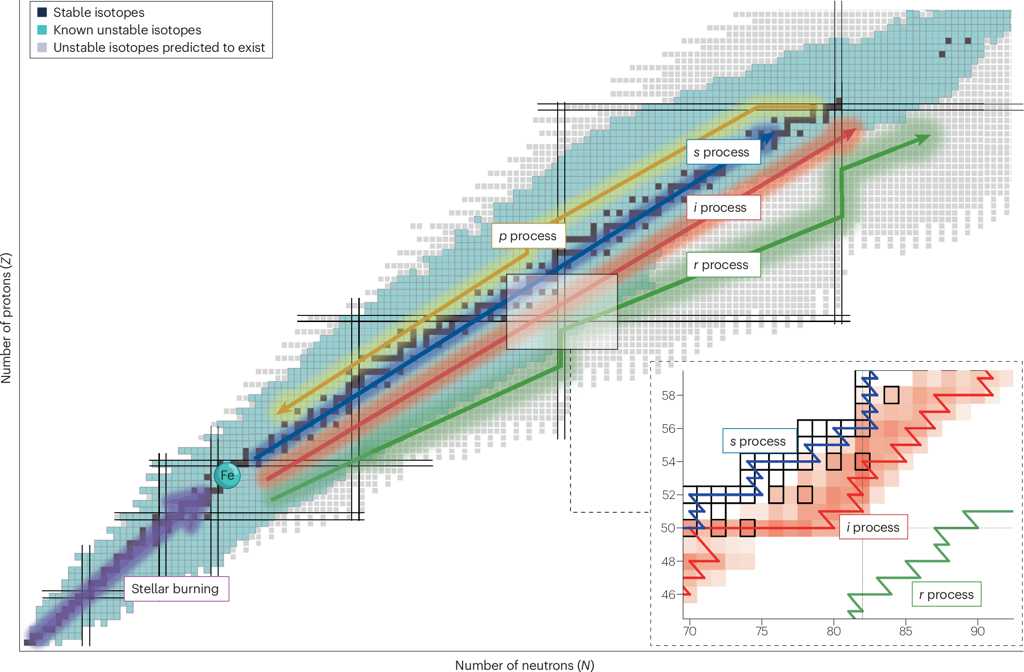
\includegraphics[width=0.5\linewidth]{astrophysicsProcesses.png}
    \caption{Diagram showing the nuclide chart with the different nucleosynthesis sites. \cite{Nature_Wiedeking}}
    \label{fig:Resonance}
\end{figure}

% the \paragraph produces a bold heading for a new paragraph but not a new subsection
\paragraph{s-process}
\paragraph{r-process}
\paragraph{p-process}


\section{Nuclear Level Density and Gamma Strength Function}

\begin{table}[]
    \centering
    \caption{Table showing the typical energy ranges for the different resonances}
    \begin{tabular}{|c|c|}
        \hline
        resonance & Typical energy range (MeV) \\
        \hline
         GDR& \\
         \hline
    \end{tabular}
    \label{tab:resonance_energy}
\end{table}


\section{TALYS}

\section{TALYS exercises} %Remember you only need to write and show plots about the exercises, not the examples. And then the last task.
The following TALYS simulations were performed using TALYS version 1.96 \cite{TALYS}. 

\subsection{Exercise 1}
\subsubsection{$\ce{^{191}Os}$}
\paragraph{$(n, γ)$}
\begin{figure}[h!]
\centering

\includegraphics[width = 0.8\textwidth]{talys_exercises/figs/Os191_n_gamma_cross_section.pdf}
\caption{Caption}
\label{fig: Os191_n_gamma_CS}
\end{figure}

\paragraph{$(n, n')$}
\begin{figure}[h!]
\centering

\includegraphics[width = 0.8\textwidth]{talys_exercises/figs/Os191_n_nprime_cross_section.pdf}
\caption{Caption}
\label{fig: Os191_n_nprime_CS}
\end{figure}


\subsubsection{$\ce{^{191}Re}$}
\paragraph{$(n, γ)$}
\begin{figure}[h!]
\centering

\includegraphics[width = 0.8\textwidth]{talys_exercises/figs/Re191_p_gamma_cross_section.pdf}
\caption{Caption}
\label{fig: Re191_p_gamma_CS}
\end{figure}


\subsection{Exercise 2}
\subsubsection{$\ce{^{208}Pb}$}
\paragraph{$(n, n')$}
\begin{figure}[h!]
\centering

\includegraphics[width = 0.8\textwidth]{talys_exercises/figs/Pb208_n_nprime_inl_cross_section_comparison_complete_data.pdf}
\caption{Caption}
\label{fig: Pb208_n_nprime_CS}
\end{figure}

\paragraph{$(n, 2n)$}
\begin{figure}[h!]
\centering

\includegraphics[width = 0.8\textwidth]{talys_exercises/figs/Pb208_n_2n_cross_section_comparison_complete_data.pdf}
\caption{Caption}
\label{fig: Pb208_n_2n_CS_EXFOR}
\end{figure}

\paragraph{$(n, γ)$}
\begin{figure}[h!]
\centering

\includegraphics[width = 0.8\textwidth]{talys_exercises/figs/Pb208_n_gamma_cross_section_comparison_complete_data.pdf}
\caption{Caption}
\label{fig: Pb208_n_gamma_CS_EXFOR}
\end{figure}


\subsection{Exercise 3}
\subsubsection{$\ce{^{208}Pb}$ With Varying Models}
\clearpage
\begin{figure}[h!]
\centering

\includegraphics[width = 1.3\textwidth,angle=-90]{talys_exercises/figs/Pb208_n_gamma_cross_section_varying_models_with_exfor.pdf}
\caption{Caption}
\label{fig: Pb208_n_gamma_var_CS_EXFOR}
\end{figure}
\clearpage


\subsection{Exercise 4}
\subsubsection{$\ce{^{191}Os}(n, γ)$ With Experimental $γ$-Ray Strength Function}
\begin{figure}[h!]
\centering

\includegraphics[width = 0.8\textwidth]{talys_exercises/figs/Os191_n_gamma_cross_section_experimental_data.pdf}
\caption{Caption}
\label{fig: Os191_n_gamma_CS_EXP}
\end{figure}


\subsection{Task}
\subsubsection{$\ce{^{120}Sn}(n, γ)$} % TODO: Better heading

test 

\section{Conclusion and Outlook}

\newpage
\section*{Appendix A: } %The * means that it will be an unnumbered section.
% you can include any appendix you want.  
\printbibliography
\end{document}

